\newpage

\section{Otimization Objective}


\quad In the process of optimization, we undertook the following steps to improve our approach:\\


Initially, we developed an evaluation function based on the statement provided by the professor. This function served as the foundation for our optimization efforts. However, we soon realized that our initial implementation was not aligned with sound software engineering practices.\\


To address this, we decided to refactor the function. Our primary objective was to introduce flexibility by allowing the specification of the number of days to evaluate. Unfortunately, due to the nature of the input, we were always limited to 7 days.\\



What set our implementation apart from others was our approach to reducing the number of variables. We concluded that since most algorithms generated values randomly, we could streamline the process by utilizing only six variables. 
We found no constraints in the provided statement that prohibited placing different beer brands within the same resource.\\


By leveraging this reduced set of variables, we were able to infer the remaining values based on the output generated by the respective algorithms. 
The analogy of playing dominoes accurately describes this approach, as each value falls into place based on the preceding one.\\


This methodology significantly minimized the need for value repairs. 
Since the values were inferred in accordance with the algorithm's output, we encountered fewer instances where, for instance, there were 100 beers in v1 resource but none in storage—a highly improbable scenario.\\


Furthermore, we established that a value range of 0 to 100 was suitable for the resources. Given that the total quantity of beers did not exceed 200, this range provided a reasonable and logical representation. Additionally, it allowed for sending a maximum of 300 units in a single day per resource, which surpassed practical requirements. By adhering to this range, the randomly generated values aligned with our expectations, ensuring meaningful results.\\


Initially, our focus revolved around maximizing profits, which required optimizing the entire function. To achieve this, we employed various algorithms, including hill climbing and Monte Carlo simulation.\\


As we shifted our attention towards minimizing the costs, we explored additional algorithms such as simulated annealing, SANN, grid search, and tabu search. However, after thorough evaluation, we concluded that Monte Carlo simulation and hill climbing emerged as the most effective algorithms for our specific problem. The alternative approaches failed to produce satisfactory results when evaluated against our optimization objectives.\\


\begin{figure}[H]
    \centering
    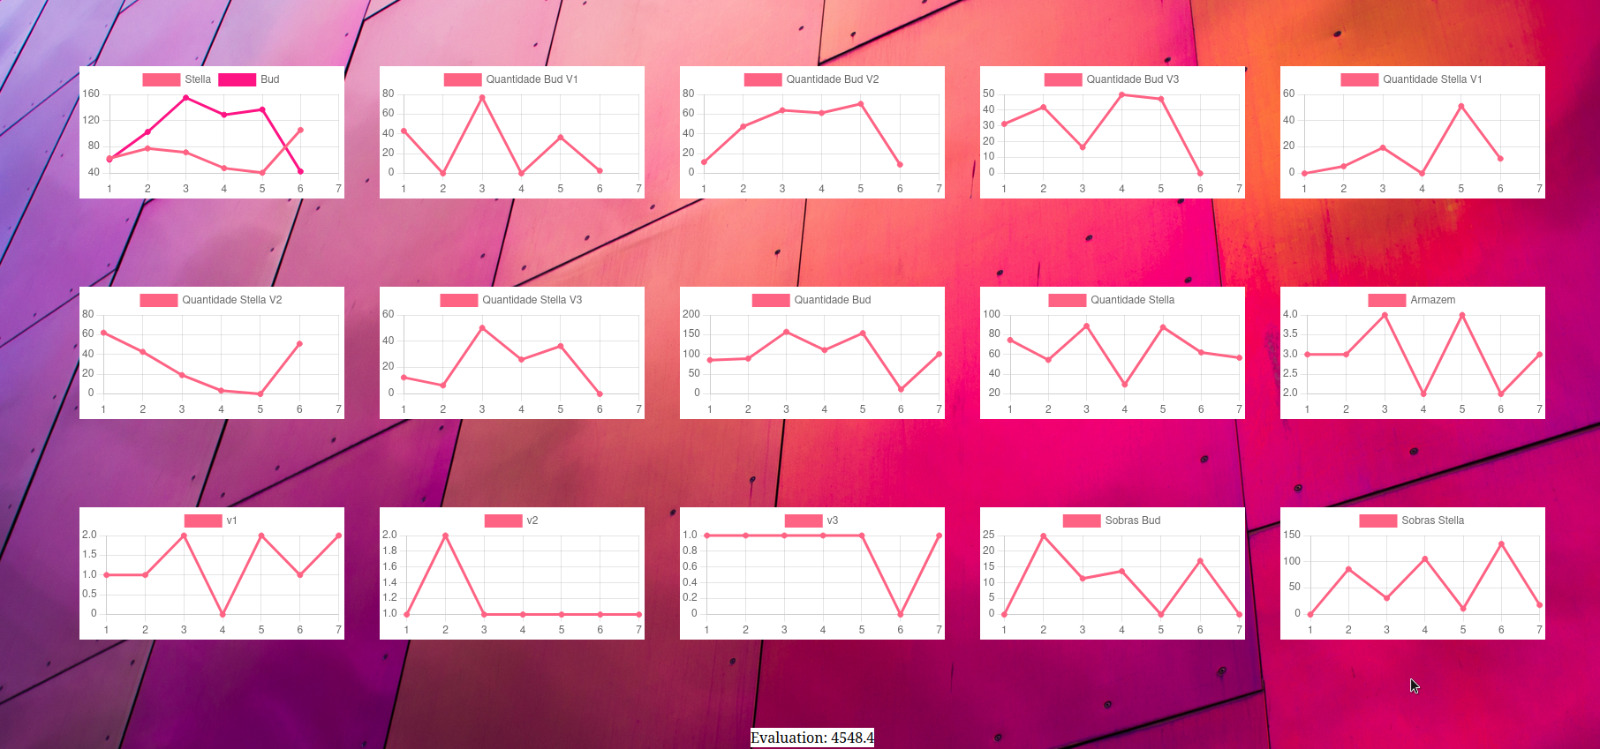
\includegraphics[width=1\textwidth]{assets/opt4.jpeg}
    \caption{Optimization maximmizing profit}
    \label{fig:stella_outliers}
    \end{figure}

\begin{figure}[H]
    \centering
    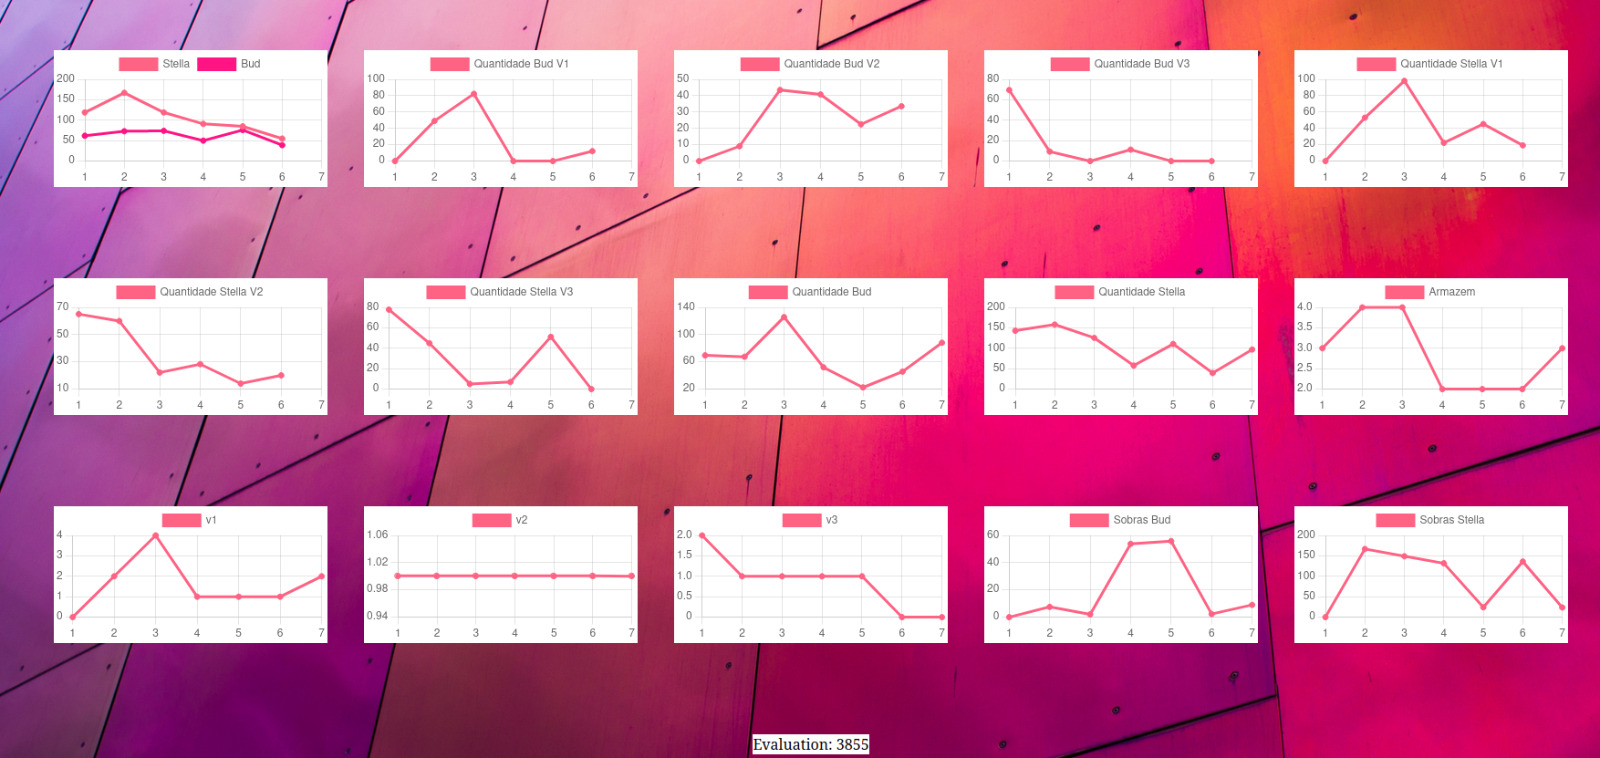
\includegraphics[width=1\textwidth]{assets/opt1.jpeg}
    \caption{Optimization maximmizing profit Montecarlo}
    \label{fig:stella_outliers}
    \end{figure}


    \begin{figure}[H]
        \centering
        
\includegraphics[width=1\textwidth]{assets/opt2.jpeg}
        \caption{Optimization minimizing costs}
        \label{fig:stella_outliers}
        \end{figure}


        \begin{figure}[H]
            \centering
            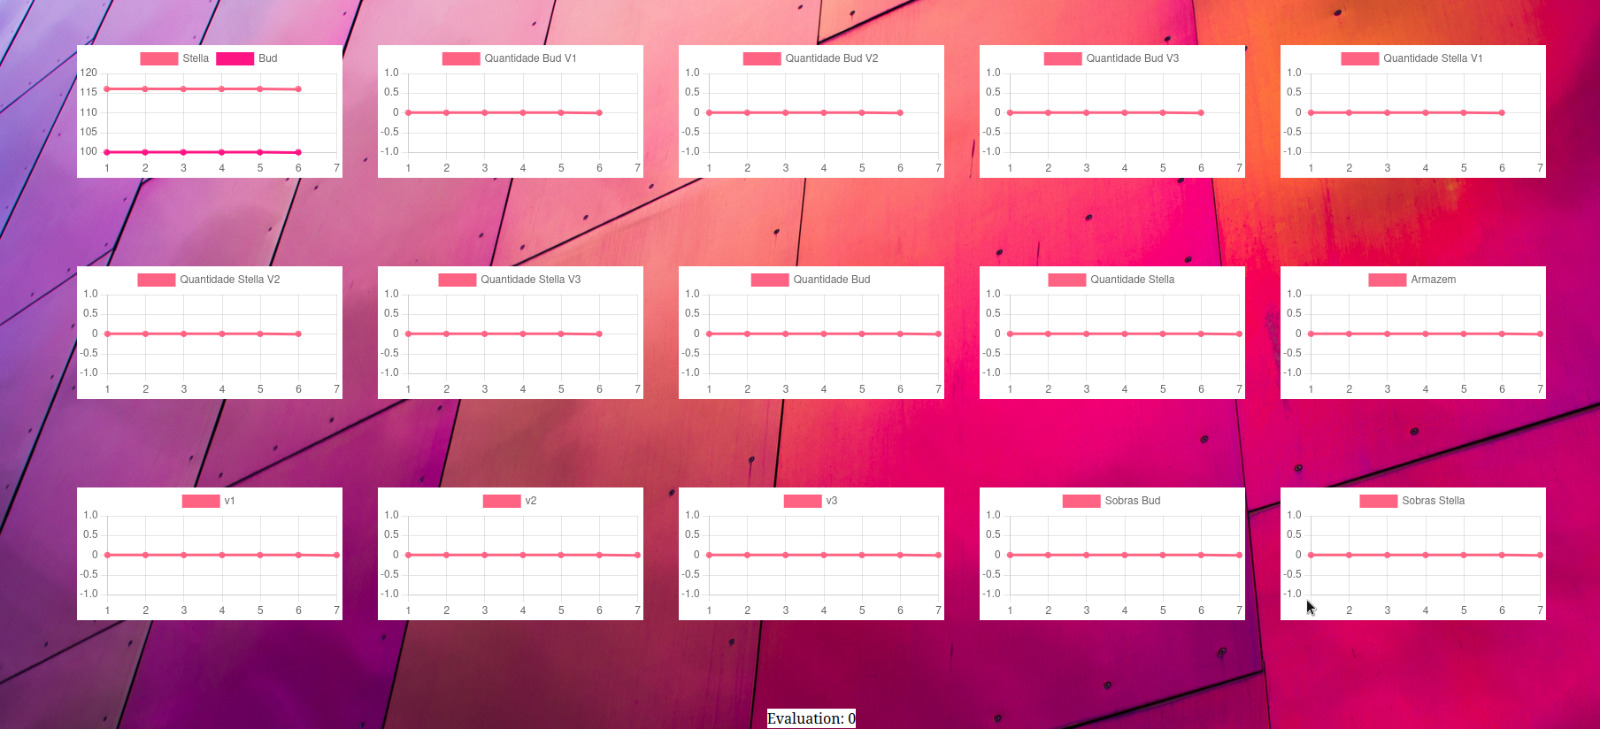
\includegraphics[width=1\textwidth]{assets/opt3.jpeg}
            \caption{Optimization minimizing costs Montecarlo}
            \label{fig:stella_outliers}
            \end{figure}


            